\chapter{Introduction and literature review}

Electrophysiological measurements of neural tissue allow direct observations of millisecond changes in neural activity, on a broad range of spatial scales from micrometers to centimeters. At these large spatial scales, electrophysiological measurements can be made entirely noninvasively through the recording of electrical potentials at the scalp. Over the last century, such scalp recordings, also known as electroencephalography (EEG), have allowed us to measure ongoing neural activity in healthy humans, as well as those suffering from neurological disease, proving itself to be a uniquely important tool for understanding the human brain. Extracting as much information as possible from these signals despite their low spatial resolution is thus highly desirable. Broadly speaking, a fundamental question is: given a difference between two EEG signals, either collected at two timepoints or from two different subjects, how much can we infer about the underlying differences in neurophysiology? 

EEG often exhibits oscillations, which are known to reflect rhythmic synchronized activity in the brain. In recent years, attention has also been devoted to the broadband trends observed in the spectra of EEG signals. In many other physical systems, such properties typically reflect second order statistical properties of the system. In EEG, it remains unclear what these broadband signals represent. Some have argued that these signals are an epiphenomenon of oscillatory brain rhythms. Others have suggested it reflects an entirely different dynamical regime of neural networks. What is the neurophysiology that underlies these broadband EEG signals? In other physical systems, the spectral trend often needs to be explicitly modelled to correct for broadband contamination of signals of interested. In EEG, it is unclear whether this is the case. Does the spectral trend contaminate brain rhythm estimates? If so, how should these signals be corrected for?

In this thesis, I address these questions through the development of biophysical and statistical models of EEG generation that integrate physiological details gleaned over the past two decades. This modelling work updates our understanding of the electric fields generated by the brain, especially as it pertains to broadband and aperiodic EEG signals. 


The physical laws that govern electric fields were described by Maxwell in the 1800s, and as such were understood well before the invention of EEG. Moreover, since the first EEG recordings, electrode and amplifier technology has improved drastically, allowing us to record signals with low noise and frequency resolutions well above that required to measure almost any neural activity. Computational power as exploded in the last decades allowing highly complex and intensive analyses of EEG signals. With these facts taken into account, it is believed that most of the remaining limits on the information available from EEG recordings are principally imposed, not by ignorance of physical laws, nor the engineering of recording systems, but primarily by our understanding of the physiological systems themselves underlying the generation of EEG signals. What do these signals represent biologically? What configurations of neural populations produce a given EEG signal?


%%%%%%%%%%%%%%%%%%%%%%%%%%%%%%%%%%%%%%%%%%%%%%%%%%%%
\section{Overview}
\label{sec:intro_overview}

\subsection{What is a T cell?}
\label{sec:intro_overview_Tcells}

At the highest level, there are two main arms of the immune system: innate and adaptive immunity. Innate immunity is the body's first line of defence against novel pathogens and is thought of as being more generalized (or non-specific); cells of the innate immune arm recognize molecular patterns that are common to many pathogens (such as polysaccharides and foreign genetic material) in order to initiate the immune response~\cite{medzhitov1997human,janeway2002innate}. Adaptive immunity, evolutionarily speaking, is much more recent, beginning to appear only in vertebrates about 500 million years ago~\cite{pancer2006evolution,redmond2018phylotranscriptomics}. In contrast to the innate immune arm, adaptive immunity is characterized by highly specific responses that are precisely tailored to the particular invading pathogen. Immunological memory, or the ability for the immune system to mount even stronger, quicker responses to a previously encountered pathogen, relies heavily on these pathogen-specific adaptive immune responses~\cite{vitetta1991memory}.

T cells, also referred to as T lymphocytes, are integral to this process of adaptive immunity. They undergo and complete their development in the \underline{t}hymus (hence their name) and carry out many important functions throughout the rest of the body (hereafter referred to as the ``periphery''). Ever since a string of studies in the 1960s led to the identification of T lymphocytes as being functionally distinct from antibody-producing B lymphocytes~\cite{mitchell1968immunological,miller1968cell,mitchell1968cell,miller2011golden}, tremendous progress has been made in elucidating just how important these cells are for recognizing and responding to different threats in a pathogen-specific manner.

Broadly, mature T cells in the periphery can be subdivided into two main classes. The first are identified via their expression of a cell surface molecule called CD8 (and are thus denoted CD8\pos{} T cells) that, when activated, become cytotoxic T lymphocytes (CTLs); these cells are also known as ``killer” T cells, so-called due their ability to recognize and kill cells infected with intracellular pathogens (of
which viruses are a prime example) as well as tumour cells~\cite{townsend1985cytotoxic,masopust2007brief,raskov2021cytotoxic,tian2022ctls}. CTLs are also heavily implicated in the pathological destruction of self-tissue during autoimmune responses~\cite{liblau2002autoreactive,walter2005cd8+}, which are described in Section~\ref{sec:intro_autoimmunity}. While alternative subsets of CD8\pos{} T cells have been described (reviewed in~\cite{mittrucker2014heterogeneity}), these have been less well characterized and will not be covered here.

The second main subdivision of T cells is instead characterized by the expression of CD4 at their cell surface; they are therefore denoted CD4\pos{} T cells. There exist many different subsets of CD4\pos{} T cells that exert separate functions (for review, see \cite{raphael2015t}), but generally speaking they are known as ``helper” T cells upon activation. For example, T-follicular helper (Tfh) CD4\pos{} T cells are necessary for providing help to B cells in producing antibodies~\cite{victora2012germinal,crotty2014t,crotty2015brief}, while type 1 helper (Th1) CD4\pos{} T cells are important for enhancing the effectiveness of innate immune cells and CTL function for intracellular pathogen clearance~\cite{del1991purified,raphael2015t,ditoro2021emerging}. Another subset of CD4\pos{} T cells, called regulatory T cells (or Tregs), are instead an immunosuppressive class of T cells; these Tregs and their functional importance will be described in further detail in Section~\ref{sec:intro_autoimmunity_peripheralTolerance}.

%%%%%%%%%%%%%%%%%%%%%%%%%%%%%%%%%%%%%%%%%%%%%%%%%%%%
\subsection{Why do we model T cells?}
\label{sec:intro_overview_modellingTcells}

Experimental tools and techniques for profiling T cells and assessing their function in various immunological contexts have undoubtedly come a long way since their discovery in the 60s. That said, even rich datasets generated from high-throughput analyses, such as multicolor flow cytometry or gene transcription profiling (RNA-seq), are often limited in their temporal resolution. In other words, while these data can provide a lot of valuable information, they generally do so at discrete snapshots in time; given the highly dynamic nature of immune responses, this can often be a limiting factor in studying them. Additionally, many of these observations can be correlative, and determining causal relationships is often not as straightforward.

Mathematical and computational modelling is therefore a great tool for bridging together some of these gaps. In particular, population models that use ordinary differential equations (ODEs) to describe immune interactions are commonly used, owing to their ease of implementation, interpretability, and predictive power for assessing causation between parameters of interest and observed outcomes. These systems of ODEs describe how population levels of, for example, effector T cells, infected host cells, and/or pathogen loads, change as a function of time, taking into account key aspects of how these variables interact with each other. With such models in hand, we can explore hypothetical scenarios by manipulating model parameters, and make predictions about how the system might behave under different conditions. This in turn can inform future experimental approaches, which may then be used to validate these predictions; thus, together, experiments and modelling can help us achieve a deeper understanding of the system under study.

While the modelling work performed in this thesis consists of differential equation modelling, including standard ODEs but also integro-differential equations and ODEs with stochastic input, one must also appreciate that other types of theoretical modelling approaches can be equally useful. For example, partial differential equations can be practical for assessing not only temporal but also spatial dynamics~\cite{su2009mathematical,moise2019rheumatoid}, and delay differential equations can explicitly incorporate non-instantaneous feedback mechanisms~\cite{bocharov1998modelling,gourley2008dynamics,fatehi2019time}. In addition to the use of differential equations, probabilistic and statistical models, agent-based models, and training of machine learning algorithms have been used to study various immunological concepts~\cite{germain2011systems,yates2014theories,eftimie2016mathematical,smith2018validated, chakraborty2017perspective}, each bringing something unique to the table but none strictly better than the other. In the sections that follow, I will attempt to illustrate the informative power of computational models by highlighting relevant examples pertaining to aspects of T cell biology under discussion. 

%%%%%%%%%%%%%%%%%%%%%%%%%%%%%%%%%%%%%%%%%%%%%%%%%%%%
\subsection{Antigen recognition -- how T cells ``see'' invading pathogens}
\label{sec:intro_overview_antigenRecognition}

In order for T cells to effectively mount an immune response against a threat, a line of communication is needed that will bridge the innate (generalized) vs. adaptive (pathogen-specific) arms of the immune system. The T cell receptor (TCR), a molecule expressed on the surface of T cells, serves this exact role. Specialized cells, called antigen-presenting cells (APCs), will phagocytose the pathogen, destroy and process it, and conjugate certain peptide fragments (on the order of 10 amino acids long) derived from pathogen proteins (i.e., ``antigens'') to major histocompatibility complex (MHC) molecules~\cite{blum2013pathways,trolle2016length,meydan2013prediction,jamaleddine2020immune}. This peptide-MHC pair (denoted henceforth as pMHC) is then trafficked to the cell surface of the APC, which migrates from the site of infection to the nearest draining lymph node~\cite{martin2009dendritic}. If a T cell whose TCRs are specific for these pMHCs then encounters and binds them at the APC surface, this, in conjunction with additional co-stimulatory and cytokine signals provided by the APC~\cite{frauwirth2002activation,curtsinger1999inflammatory,curtsinger2010inflammatory}, then triggers a cascade of events that lead to T cell activation, differentiation, proliferation, and effector function (Fig.~\ref{fig:intro_TcellActivation}).

\begin{figure}[b!]
    \centering
    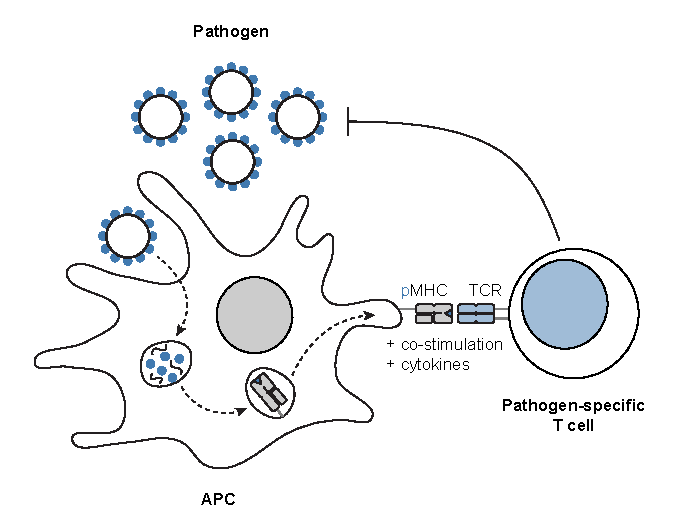
\includegraphics[width=0.64\textwidth]{Figures/intro/fig1_TcellActivation.pdf}
    \caption[Overview of T cell activation via antigen recognition]{\captiontitle{Overview of T cell activation via antigen recognition.} Antigen presenting cells (APCs) phagocytose pathogens and degrade them via proteolytic pathways. Peptide fragments derived from proteins/antigens of the processed pathogen are then coupled to MHC molecules to form peptide-MHC (pMHC) pairs, which are then shuttled to the APC surface. The binding of specific T cell receptors (TCRs) to these pMHC ligands expressed on APCs then trigger, in the presence of co-stimulatory molecules and cytokines produced by APCs, T cell activation and proliferation needed for pathogen control.}
    \label{fig:intro_TcellActivation}
\end{figure}

At this stage, it should be noted that there are two main forms of MHC that we will consider\footnote{Other, non-antigen presenting classes of MHC exist but will not be covered here; for reviews see~\cite{colten1984expression,gruen2001human}.}: they are MHC class I (MHCI), recognized by CD8\pos{} T cells and presenting peptides between 8-15 but usually 9 amino acids long~\cite{trolle2016length,meydan2013prediction}, and MHC class II (MHCII), recognized by CD4\pos{} T cells~\cite{rock2016present} and presenting longer peptides up to 30 amino acids in length~\cite{meydan2013prediction}. The expression of MHCII is restricted to APCs (including dendritic cells, macrophages, and B cells), while all nucleated cells in the body express MHCI~\cite{hewitt2003mhc,van2011expression,rock2016present}. When a cell is infected by an intracellular pathogen, its cellular machinery will conjugate pathogen-derived peptides to MHCI, thus flagging itself for elimination by cytotoxic CD8\pos{} T cells~\cite{rock2016present}.

The importance of the TCR for adaptive immunity cannot be overstated, as the ability of T cells to play out their roles rely crucially on this initial TCR:pMHC interaction. TCRs thus act as the ``eyes'' of the adaptive immune system; only those TCRs that can bind to the pathogen-specific pMHC with adequate strength (in other words, with sufficient ``reactivity'') will become activated and initiate a targeted response to that pathogen. What exactly is meant, from a functional standpoint, by a TCR being ``specific'' for a given pMHC (termed its ``cognate'' pMHC) will be the focus of the next section.

%%%%%%%%%%%%%%%%%%%%%%%%%%%%%%%%%%%%%%%%%%%%%%%%%%%%
\subsection{Antigen discrimination -- how T cells ``know'' when to respond}
\label{sec:intro_overview_antigenDiscrimination}

At homeostasis, all nucleated cells in an organism express pMHC where the ``p'' is a peptide derived from endogenous proteins found throughout the body~\cite{hewitt2003mhc,van2011expression,rock2016present}; these are called self-pMHCs, and, under healthy conditions, normal protein processing pathways within cells lead to baseline self-pMHC expression. In fact, both CD4\pos{} and CD8\pos{} T cells need to receive sub-threshold signals from self-pMHC on APCs to survive long-term in the periphery~\cite{takeda1996mhc,brocker1997survival,kirberg1997peripheral,tanchot1997differential}. An apparent dilemma thus arises: given that all TCRs must bind self-pMHC to some extent, how does an activation threshold manifest itself from a continuous range of TCR:pMHC binding strengths, such that a T cell responds only to pathogen-derived \textit{foreign}-pMHC in a specific yet sensitive way? In other words, how do T cells become activated when presented with foreign antigen even at low concentrations (sensitivity) but remain neutral in the presence of constant and abundant self-pMHC (specificity)? Impressively, it has been shown that even a very small number of pMHC molecules is required for T cell activation~\cite{irvine2002direct}, with as few as one single pMHC ligand being sufficient to induce a measurable T cell response~\cite{huang2013single} provided that the TCR is specific for it. Thus, T cells searching for their cognate pMHC ligand is akin to searching for a needle in a haystack, yet they have remarkably evolved to do exactly that.

Our understanding of just how TCRs can effectuate such exquisite discrimination between self and non-self antigens has greatly benefited from mathematical modelling efforts~\cite{feinerman2008quantitative,franccois2016case}. In 1995, Timothy McKeithan proposed a now-famous conceptual model of immune recognition using the ``kinetic proofreading'' (KPR) principle~\cite{mckeithan1995kinetic}. Briefly, this model assumes that a TCR and pMHC must be bound long enough for TCR-associated intracellular molecules to undergo $N$ successive phosphorylation steps (or modifications), and that only at this stage do downstream signaling processes occur leading to T cell activation. An interesting finding of this model is that, if this theoretical number $N$ is large enough, then even small differences in TCR:pMHC binding duration can lead to large differences in the proportion of complexes that can achieve all $N$ modifications (Fig.~\ref{fig:intro_KPR}). Thus, within this KPR framework, the TCR may theoretically achieve sensitivity for pMHC that it is ``specific'' for while remaining tolerant to others. Recently, Tischer and Weiner used optogenetics to specifically modulate how long the TCR remained bound to antigen~\cite{tischer2019light}; consistent with the KPR principle, they showed that tuning the duration of binding indeed generates a sharp threshold of T cell activation.

\begin{figure}[ht]
    \centering
    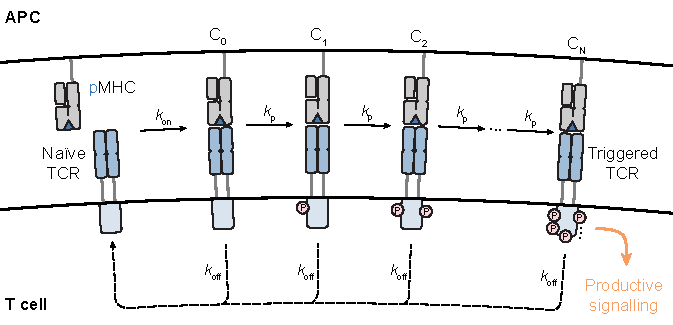
\includegraphics[width=0.64\textwidth]{Figures/intro/fig3_KPR.pdf}
    \caption[Schematic of the kinetic proofreading model for T cell activation]{%
    \textit{Schematic of the kinetic proofreading model for T cell activation}. %
    According to this model, the TCR binds pMHC at a rate $k_{\textup{on}}$ to form a TCR:pMHC complex, $C_0$. While bound, intracellular domains associated with the TCR undergo modifications via phosphorylation at a rate $k_{\textup{p}}$, causing the complex to transition from state $C_i$ to $C_{i+1}$ ($i=0,1,2,..., N-1$), where each transition represents one modification step. Unbinding of the TCR:pMHC complex (at a rate equal to $k_{\textup{off}}$) rapidly reverses these modifications, causing the TCR to revert back to its ``na\"{i}ve'' unbound state. The TCR is assumed to become ``triggered'' only when it undergoes all $N$ modification steps; triggered TCRs then initiate downstream activation and response. The TCR is specific for the pMHC only if the duration of binding is sufficiently long enough to trigger a response. Adapted from~\cite{mckeithan1995kinetic}.}
    \label{fig:intro_KPR}
\end{figure}

In reality, the downstream processes that lead to T cell activation involve a fairly complex biochemical series of events (the details of which lie outside the scope of this thesis; for recent reviews, see~\cite{hwang2020recent,shah2021t}), but importantly $N$ successive modifications proposed by the model can indeed be likened to phosphorylation of immunoreceptor tyrosine-based activation motif (ITAM) sites on the cytoplasmic molecules that complex with the TCR and that are responsible for downstream signal transduction~\cite{vstefanova2003tcr,love2010itam}. Subsequent studies have built upon the KPR principle to incorporate additional aspects of TCR signalling downstream. For example, Altan-Bonnet and Germain developed a detailed biochemical model showing that a combination of positive and negative feedback loops could better achieve sensitivity and specificity for its ligand~\cite{altan2005modeling}. Fran\c{c}ois et al. later showed that even a very simple, phenotypic model incorporating negative regulation to the KPR scheme can reproduce the speed, specificity, and sensitivity required for TCR antigen discrimination, even for smaller numbers of modification steps~\cite{franccois2013phenotypic}.

Other studies have used modelling to suggest additional ways by which TCRs achieve the sensitive and specific recognition of its cognate ligand. In one such case, Dushek and van der Merwe proposed that pMHC ``rebinding'' within the kinetic proofreading scheme can improve antigen discrimination by T cells, for example by inducing the formation TCR nanoclusters  on the T cell surface in such a way that the pMHC is more likely to rebind TCRs as a function of nanocluster size~\cite{dushek2014induced}. In another model, Ganti et al. argue using principles derived from information theory that spatial localization of feedback signals relative to the TCR plays a role, postulating that early negative feedback in physical proximity to the TCR are important for sensitive antigen discrimination, while more distal, late positive feedback serves the purpose of signal amplification post-discrimination~\cite{ganti2020t}.

%%%%%%%%%%%%%%%%%%%%%%%%%%%%%%%%%%%%%%%%%%%%%%%%%%%%
\subsection{T cell proliferation -- raising an army}
\label{sec:intro_overview_proliferation}

Upon interaction with an APC bearing its cognate pMHC, the newly-activated T cell must undergo several rounds of division. The result is exponential growth, with final numbers of activated T cells expanded by several orders of magnitude relative to the number of pre-activated, or ``na\"{i}ve'', T cell precursors. For example, in the case of T cells specific for lymphocytic choriomeningitis virus (LCMV)\footnote{In particular, this study quantified GP$_{33}$-specific CD8\pos{} T cells; these are T cells whose TCRs bind MHC conjugated to a peptide fragment derived from the LCMV viral glycoprotein (GP), starting from position 33 of the GP amino acid sequence up to position 41.}, it was determined that 100-200 na\"{i}ve precursors in mice expand to a staggering $\sim$10 million cells one week post-infection~\cite{blattman2002estimating}. This process of antigen-driven T cell proliferation of a single T cell population has been mathematically described by de Boer and Perelson in 1995~\cite{de1995towards}, who, from a simple kinetic scheme of T cell binding to antigen, derived the following equation:
%
\begin{equation}
    \dv{T}{t} = \sigma + \rho \, T \frac{P}{P + \flatfrac{1}{K} + T} - \delta \, T.
    \label{eq:intro_deboer1995}
\end{equation}
%
Here, $T$ denotes the number of T cells, while $\dv*{T}{t}$ represents the rate of change of this number with respect to time. The term $\sigma$ represents a constant influx of new na\"{i}ve T cell precursors from the thymus, while $\delta$ represents the \textit{per capita} death (i.e., turnover) rate of T cells. The middle term represents the effect of T cell division in the presence of antigen at a concentration $P$, with a maximum \textit{per capita} proliferation rate $\rho$ with the quantity $K$ representing the overall strength of binding of the T cell with the APC -- this parameter is also called T cell ``avidity'' (see Section~\ref{sec:intro_affinity_TcellAvidity}).

This model, while simple and with only a few parameters, provides important insight into key features of T cell replication. First note that, in the absence of cognate pMHC (i.e., when $P=0$), a steady-state level of precursor T cells is reached when $T = \flatfrac{\sigma}{\delta}$; this is obtained by setting Eq.~\eqref{eq:intro_deboer1995} to 0 and solving for $T$, and represents the number antigen-specific T cells at homeostasis (e.g., the 100-200 LCMV precursors). Upon introduction of pathogen, when $P$ is large and $T$ is still small, exponential growth in the number of T cells is observed, hence the number of antigen-specific T cells may grow to very large numbers (e.g., to the 10 million observed a week post-infection with LCMV). Furthermore, the function representing T cell proliferation saturates at high concentrations of cognate pMHC, eventually plateauing at an upper-bound determined by $\rho$. Finally, the additional $T$ term in the denominator represents competition for antigen binding sites between T cells; it becomes important when multiple clones of T cells are considered simultaneously, as it prevents the T cell population in the model from growing unboundedly.

This formalism for T cell proliferation has since been adapted for use in many other population models of effector T cells in various contexts, including those presented in~\cite{de1998target,khadra2009role,khadra2011investigating,conway2015post,mayer2019regulation} developed over a period spanning nearly 30 years. Importantly, this formalism describing T cell expansion in the presence of cognate antigen is adapted in our own models presented in Chapters~\ref{sec:Tr1}-\ref{sec:VE} of this thesis.

%%%%%%%%%%%%%%%%%%%%%%%%%%%%%%%%%%%%%%%%%%%%%%%%%%%%
\subsection{The generation of TCR repertoire diversity}
\label{sec:intro_overview_TCRdiversification}

Conservative estimates put the number of potential antigens that an organism could theoretically encounter throughout its life on the order of trillions, though the true number could very well be several orders of magnitude more than even this~\cite{mason1998very,yates2014theories}. Given this enormous variety, a mechanism needs to be put in place to generate a sufficient number of unique TCRs so as to be able to cover the sheer breadth of potential antigens that the host may encounter.

Each T cell expresses many copies (on the order of $10^4$) of a unique TCR on its surface~\cite{labrecque2001much}. The collection of all T cells bearing the same TCR is called a T cell clonotype, while the collection of all unique TCRs within an organism is termed its TCR ``repertoire''. Structurally, the TCR is a heterodimer, with most circulating T cells being formed from a TCR\textalpha{} and a TCR\textbeta{} chain; these are termed \textalpha{}\textbeta{}~T cells.\footnote{A small subset of circulating T cells, present at a frequency of $\sim$1-5\% in adult humans and mice~\cite{lanier1988structural,groh1989human}, are instead formed from a \textgamma{}- and a \textdelta{}-chain. These \textgamma{}\textdelta{}~T cells are present at higher frequencies in the skin and gut and, while interesting in their own right, will not be covered in this thesis -- for a review of \textgamma{}\textdelta{}~T cells and their function, see~\cite{vantourout2013six}.} Early estimation of the number of unique \textalpha{}\textbeta{}~T cell clonotypes determined a lower bound of 25 million unique TCRs in the human body, with true diversity certain to exceed this figure~\cite{arstila1999direct}. The number of protein-coding genes in the human genome, on the other hand, is only about 20 thousand~\cite{salzberg2018open,piovesan2019human}. Thus, there cannot be a one-to-one correspondence between a gene and a unique TCR\textalpha{} or TCR\textbeta{} chain. Instead, jawed vertebrates have evolved a clever process to generate large T and B lymphocyte receptor diversities, called V(D)J recombination~\cite{litman2010origins}.

The T and B cell antigen receptors coded by the germline DNA (i.e., the inherited version of those genes) are non-functional prior to lymphocyte development; instead, they are composed of many V and J segments, with the germline TCR\textbeta{} gene also containing 2 additional D segments in the case of T cells~\cite{litman2010origins,schatz2011recombination}. During T cell development in the thymus, recombination-activating gene (RAG) protein complexes mediate the semi-random combination of these V and J (for the TCR\textalpha{} chain), or V, D, and J (for the TCR\textbeta{} chain), segments~\cite{schatz2011recombination,robins2010overlap}, generating massive diversity from the sheer number of possible combinations of these segments. Additionally, during RAG-mediated joining of each pair of segments, a unique DNA polymerase called terminal deoxynucleotidyl transferase (henceforth referred to as TdT) inserts an average of 2 to 5 non-templated (simply put: random) nucleotides, or ``N-nucleotides'', into the junctions between these segments~\cite{schatz2011recombination,mickelsen1999modulation}\footnote{The functional role of N-diversification by TdT will be investigated further in Chapters~\ref{sec:AvC} and~\ref{sec:VE}.}. Finally, pairing of the new TCR\textbeta{} chain (which undergoes recombination first) to the new TCR\textalpha{} chain to form the TCR heterodimer further increases the number of possible TCRs, with at least 25 TCRs, on average, sharing the same TCR\textbeta{} chain while differing via distinct TCR\textalpha{} chains~\cite{arstila1999direct}. The mechanisms of TCR repertoire diversification are summarized in Fig.~\ref{fig:intro_TCRdiversity}. Together, these processes combined were estimated to generate an astounding $10^{15}$ to $10^{20}$ unique TCRs~\cite{davis1988t,zarnitsyna2013estimating}; to put into context just how massive this number is, the number of grains of sand in all the beaches and deserts on Earth, approximately 7.5\E{18}~\cite{blatner2012spectrums}, falls squarely within this range.

\begin{figure}[ht]
    \centering
    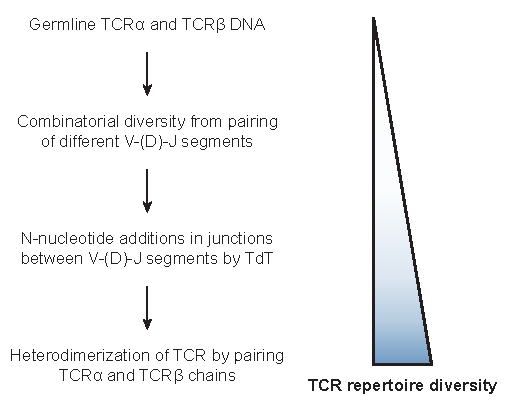
\includegraphics[width=0.48\textwidth]{Figures/intro/fig2_TCRdiversity.pdf}
    \caption[Summary of TCR repertoire diversification]{%
    \textit{Summary of TCR repertoire diversification}. %
    Combinatorial diversity is achieved by random joining of V, (D,) and J segments recombination, N-nucleotide addition, and heterodimerization of TCR\textalpha{} and TCR\textbeta{} chains.}
    \label{fig:intro_TCRdiversity}
\end{figure}

The ``realized'' repertoire diversity of T cells, however, is certainly smaller than this theoretical maximum. For one, there are about 400 billion T cells throughout the human body~\cite{jenkins2009composition}; $10^{15}$ T cells, on the other hand, would weigh about half a metric tonne~\cite{lythe2016many}. Extrapolating, $10^{20}$ T cells would weigh around 50,000 tonnes, more than four times the weight of the Eiffel Tower. Second, there exist many T cell clonotypes composed of multiple T cells with identical TCRs~\cite{robins2009comprehensive,quigley2010convergent,zarnitsyna2013estimating,qi2014diversity,de2020naive}. Third, V(D)J recombination is not totally random, as it is known that there are intrinsic biases in segment usage and N-nucleotide additions by TdT~\cite{robins2010overlap,murugan2012statistical}, and redundancies in protein encoding would mean that different genetic sequences could converge to the same TCR protein structure~\cite{quigley2010convergent}. Fourth, not all rearranged TCRs will live to see the light of day owing to harsh selection processes in the thymus. Specifically, once the developing T lymphocyte has successfully rearranged its TCR, that new TCR must be tested for its ability to bind self-pMHC sufficiently (ensuring that the TCR is functional and useful) but not excessively (to prevent autoimmune responses). The processes of positive and negative selection in the thymus, respectively, are the mechanisms that ensure these two conditions are met~\cite{yates2014theories,klein2014positive,kondo2019thymus}. Together, these checkpoints purge about 95\% or more of T cells before they can become fully fledged mature na\"{i}ve T cells in the periphery~\cite{kyewski2006central}.

Estimates from TCR sequencing data on the realized TCR diversity in adult humans range from $10^7$ to $10^8$ unique TCR clonotypes~\cite{robins2009comprehensive,qi2014diversity,de2020naive}. Incidentally, there are many technical challenges involved in measuring realized TCR repertoire diversity across all T cells of the body~\cite{zarnitsyna2013estimating,mora2019many} which involves extrapolation of data obtained from a comparatively small subset of all TCRs (a truly non-trivial task). Stochastic models have therefore been used to infer T cell clonotype distributions, and consequently the number of T cell clones, based on homeostatic processes such as thymic input, division, cell death, and competition for self-pMHC~\cite{desponds2016fluctuating,lythe2016many,mora2019many}. In particular, Lythe et al. used such a model to propose that the number of T cell clonotypes may be much higher than previous estimates, finding that this number may only be about 10-fold lower than the total number of T cells~\cite{lythe2016many} in the periphery, i.e., on the order of $\sim$10 billion ($10^{10}$) in humans.

%%%%%%%%%%%%%%%%%%%%%%%%%%%%%%%%%%%%%%%%%%%%%%%%%%%%
\subsection{Summary and highlights}

The concepts of TCR diversification, antigen recognition/discrimination, and pMHC binding strengths have important implications for T cell responses, and thus for proper immune function. At one extreme, failure of T cells to discriminate between self- and foreign-pMHC can lead to the development of autoimmune disorders. What mechanisms exist to prevent their manifestation, and under what conditions these mechanisms may fail, will be discussed in Section~\ref{sec:intro_autoimmunity}. At the other extreme, failure of T cells to recognize and respond to foreign pathogens can lead to immunodeficiency and immune escape. The mechanisms used by pathogens to evade T cell recognition will be discussed in Section~\ref{sec:intro_immuneEscape}. Between these two extremes, T cells recognize foreign-pMHC with varying degrees of sensitivity lying within a continuum of binding strengths. How this continuum is defined, and how it may shape the anti-microbial T cell response, will be discussed in Section~\ref{sec:intro_affinity}.

%%%%%%%%%%%%%%%%%%%%%%%%%%%%%%%%%%%%%%%%%%%%%%%%%%%%
%%%%%%%%%%%%%%%%%%%%%%%%%%%%%%%%%%%%%%%%%%%%%%%%%%%%

\section{T cell tolerance and autoimmunity}
\label{sec:intro_autoimmunity}

As mentioned in Section~\ref{sec:intro_overview_antigenDiscrimination}, self-pMHC is present throughout the entire body. The question becomes: how are T cells, which rearrange their TCR and undergo selection processes in the thymus, supposed to be trained not to become activated by self-pMHC in the periphery? Training T cells to remain ``tolerant'' to self is critical, as TCR signal strengths resulting from interactions with self-pMHC that are too strong can lead to T cell activation and immune-driven destruction of healthy endogenous tissue --  a hallmark of autoimmunity. Indeed, autoimmune disorders, like any adaptive immune response, are believed to be T cell mediated; examples where this is known include, but are not limited to, type 1 diabetes mellitus, rheumatoid arthritis, multiple sclerosis, Hashimoto's disease, autoimmune hepatitis, inflammatory bowel disease, and systemic lupus erythematosus~\cite{giwa2020current,weyand2020immunometabolism,liu2022autoreactive,chistiakov2005immunogenetics,sirbe2021pathogenesis,imam2018effector,sharabi2020t}.

In all cases, autoimmune T cell responses arise in contexts where the mechanisms of self-tolerance fail. Broadly, the checkpoints in place to prevent autoimmunity belong to one of two categories: central tolerance, or peripheral tolerance. What these are, and how they work to circumvent the development of autoimmune disorders via autoreactive T cells will be the focus of this section. Note that the concept of T cell tolerance is broad and can extend beyond the context of self-antigens to include, for example, tolerance to commensal microbes that constitute the symbiotic microbiome~\cite{nutsch2012t}, or exhaustion in the context of chronic infections or cancer~\cite{schietinger2014tolerance} (a concept that will be revisited in Section~\ref{sec:intro_immuneEscape_mechanisms}). The remainder of this section, however, will focus specifically on the establishment (or failure) of tolerance to self in the context of autoimmunity.

%%%%%%%%%%%%%%%%%%%%%%%%%%%%%%%%%%%%%%%%%%%%%%%%%%%%
\subsection{Central tolerance -- the role of negative selection}
\label{sec:intro_autoimmunity_centralTolerance}

Central tolerance comprises the set of processes during T cell development within the thymus that aim to eliminate autoreactive T cells whose rearranged TCRs bind self-pMHC too strongly (thus having the potential to become activated in the periphery in response to antigens derived from the host's own tissue). This process is termed negative selection, and was touched upon briefly in Section~\ref{sec:intro_overview_TCRdiversification}.  After developing T cells have undergone V(D)J recombination for both chains of their TCR and have passed through positive selection in the cortical region of the thymus, they migrate to the thymic medulla~\cite{takahama2006journey,love2011signal}. There, a specialized subset of medullary thymic epithelial cells (mTECs), together with dendritic cells (a professional APC) and thymus-resident B cells, will present a large library of self-antigens derived from proteins expressed throughout the entire body~\cite{klein2014positive,takahama2006journey,love2011signal,castaneda2021multifaceted}. While some of these self-antigens may be found ubiquitously throughout the body (since they are derived from proteins expressed in many or all cell types), others may only be expressed in very specific organs and are hence referred to as ``tissue-restricted'' antigens (TRAs)~\cite{kyewski2006central,kondo2019thymus}.

If a T cell, via its TCRs, binds too strongly to self-pMHC in the thymus that it could potentially re-encounter in the periphery, this leads to one of two potential outcomes~\cite{kondo2019thymus}. In the first case, the T cell is deleted by apoptosis (i.e., programmed cell death) and thus prevented from escaping the thymus and becoming part of the mature na\"{i}ve T cell pool. In the second, however, the T cell is instead destined to become a regulatory T cell or Treg (specifically, a ``natural'' Treg, in contrast to ``induced'' Tregs which will be discussed in Section~\ref{sec:intro_autoimmunity_Tregs}). Tregs, as mentioned in Section~\ref{sec:intro_overview_Tcells}, differ from conventional T cells in that they instead primarily play an immunosuppressive (as opposed to a pro-inflammatory) role. The result is thus an immunosuppressive T cell that binds self-pMHC more strongly, on average, than circulating conventional T cells~\cite{tanaka2010graded,killebrew2011self,moran2011t,li2016t}. Which of these two fates (apoptosis or diversion to the Treg lineage) awaits a given autoreactive T cell in the thymus is still not completely understood, though this is likely a result of multiple factors. For one, it was shown that self-pMHC expression patterns in the thymus can influence this outcome, where higher expression levels favour clonal deletion while lower expression levels favour the production of Tregs~\cite{malhotra2016tolerance}. Additionally, there is evidence to suggest that intrinsic properties of the TCR itself might play a role, given that the genetic sequences that make up the TCRs of conventional vs. regulatory T cells were shown to be distinct (though with some degree of overlap)~\cite{hsieh2004recognition,wong2007adaptation,savage2020regulatory}.

The ability for mTECs to express pMHC that might only be found, for example, in the kidney or in the pancreas, is known as promiscuous gene expression and is key to establishing central tolerance. This function is largely (though not exclusively) mediated by a unique transcription factor known as autoimmune regulator (AIRE)~\cite{derbinski2005promiscuous,kyewski2006central}. Indeed, people with mutations in the gene encoding AIRE, leading to deficiency in AIRE expression, present with severe multiple-organ autoimmunity~\cite{betterle1998autoimmune,anderson2005cellular,besnard2021aire}, thus highlighting the crucial role of central tolerance mechanisms in preventing autoimmune disorders. 


%%%%%%%%%%%%%%%%%%%%%%%%%%%%%%%%%%%%%%%%%%%%%%%%%%%%
\subsection{Peripheral tolerance -- ignorance, anergy, and regulation}
\label{sec:intro_autoimmunity_peripheralTolerance}

Central tolerance in the thymus allows for the detection and deletion of autoreactive T cells before they have the opportunity to encounter their cognate antigen, derived from self, in the periphery. However, it has been established that central tolerance is a fairly incomplete process, and that a sizeable fraction of autoreactive T cells ($\sim$1/3) do escape negative selection to become part of the mature na\"{i}ve T cell repertoire~\cite{bouneaud2000impact,gallegos2006central,eltanbouly2021rethinking}. Therefore, while necessary, central tolerance alone is not sufficient for curtailing autoimmune responses. Accordingly, additional mechanisms must be put in place in order to prevent the development of autoimmune disease; these additional mechanisms fall under the umbrella of peripheral tolerance.

T cell ignorance is perhaps the first facet of peripheral tolerance specifically keeping autoreactive T cells in check~\cite{salaman2020breakdown,eltanbouly2021rethinking}. Conventional na\"{i}ve CD4\pos{} and CD8\pos{} T cells, including those that are autoreactive, exit the thymus in a quiescent state~\cite{chapman2020metabolic}; as described in Section~\ref{sec:intro_overview_antigenDiscrimination}, these T cells only exit quiescence if their TCR comes into contact with their cognate pMHC and the stability and duration of this interaction is sufficient to trigger T cell activation. However, perhaps due to autoreactive T cells having TCRs that bind their cognate self-antigen less strongly~\cite{zehn2006t,leube2023single} in combination with low abundance of (and/or restricted access of these T cells to) their cognate self-antigens~\cite{kurts1999cd8,eltanbouly2021rethinking}, they may fail to become activated in the periphery (Fig.~\ref{fig:intro_peripheralTolerance}A). 

\begin{figure}
    \centering
    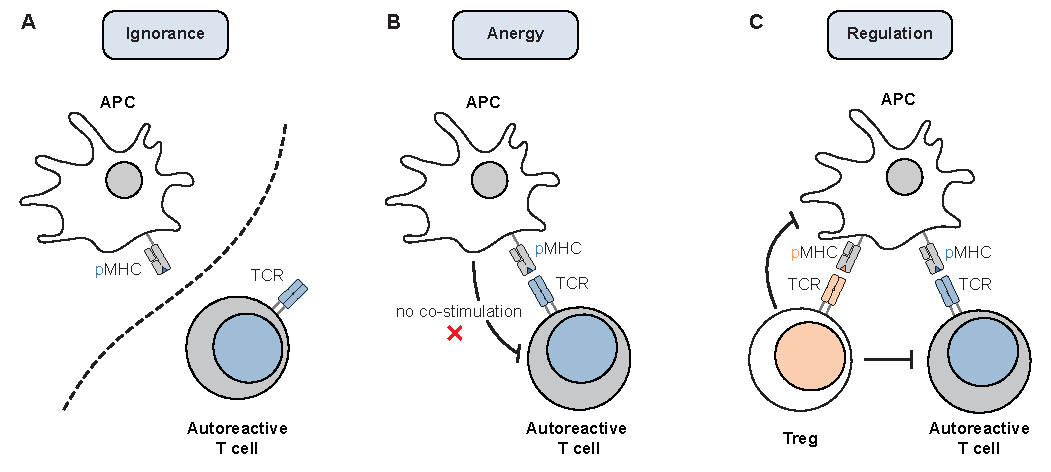
\includegraphics[width=\textwidth]{Figures/intro/fig4_peripheralTolerance.pdf}
    \caption[Summary of peripheral tolerance mechanisms]{%
    \textit{Summary of peripheral tolerance mechanisms}. %
    \secbfcolor{(A)}~T cell ignorance occurs when an autoreactive T cell fails to activate in the periphery, owing to restricted access of its TCR to its cognate pMHC on APCs, and/or no/low self-antigen abundance in conjunction with low TCR:pMHC binding strengths. %
    %
    \secbfcolor{(B)}~T cell anergy (hyporesponsiveness) is induced upon TCR:pMHC engagement in the absence of co-stimulatory signals from the APC. %
    %
    \secbfcolor{(C)}~Regulatory T cells (Tregs) use a number of mechanisms to suppress autoreactive T cell activation, acting both directly on those T cells or by impairing the ability of APCs to activate them.}
    \label{fig:intro_peripheralTolerance}
\end{figure}

The next line of defence in the peripheral tolerance arsenal is the induction of autoreactive T cell anergy. Briefly, anergy is defined as a long-lasting hyporesponsive state following cognate antigen encounter~\cite{schwartz1989t,schwartz2003t,appleman2003t,eltanbouly2021rethinking}. As mentioned in Section~\ref{sec:intro_overview_antigenRecognition}, the TCR:pMHC interaction is necessary but not sufficient to induce T cell activation and proliferation~\cite{lafferty1978immunological,mueller1989accessory}. In fact, in the absence of co-stimulation through accessory surface proteins on the APC (e.g., B7-1 or B7-2) engaging their ligands on the T cell (e.g., CD28), T cell activation fails and the T cell is rendered unresponsive even to subsequent antigen stimulation~\cite{ragazzo2001costimulation,wells2001signaling}. It should be noted that there is considerable phenotypic diversity with regard to transcriptional states in anergic T cells (reviewed in~\cite{valdor2013induction}) as well as different molecular mechanisms that can induce distinct forms of T cell anergy~\cite{wells2001signaling}. In any case, the bottom line is that these autoreactive T cells are prevented from becoming fully-fledged effector T cells, thus sparing the organism from damaging autoimmune responses (Fig.~\ref{fig:intro_peripheralTolerance}B).

Another crucial contributor to the establishment of peripheral tolerance, and the focus of the remainder of this section, is the regulatory T cell (Treg). Although these immunosuppressive T cells can exert their effect in several distinct ways~\cite{sakaguchi2008regulatory,shevyrev2020treg}, it was shown that, like conventional T cells, many Treg functions rely on the ability of their TCR to engage self-pMHC in the periphery~\cite{levine2014continuous,vahl2014continuous,schmidt2015regulatory}. In addition to serving the important role of peripheral tolerance to self-antigens, Tregs also induce tolerance to microbiome-derived, food-derived, and fetus-derived antigens, and are involved in tissue regeneration post-injury~\cite{xu2018c,zhang2001activation,burt2013fetal,shevyrev2020treg}. An overview of different types of regulatory T cells, as well as a summary of ways in which these Tregs exert their immunosuppressive effects in the context of peripheral tolerance to self-antigens, will be provided in the next section.

%%%%%%%%%%%%%%%%%%%%%%%%%%%%%%%%%%%%%%%%%%%%%%%%%%%%
\subsection{Regulatory T cells -- subsets and mechanisms of action}
\label{sec:intro_autoimmunity_Tregs}

Typically, the name Treg is used interchangeably with CD25\pos{} CD4\pos{} T cells expressing FOXP3, the master transcriptional regulator of Treg cell development and function. These can be further divided into natural Tregs (nTregs) that already express FOXP3 and possess an immunoregulatory phenotype upon egress from the thymus, vs. induced Tregs (iTregs) that begin as conventional CD25\neg{}~CD4\pos{} T cells and acquire FOXP3 expression and immunoregulatory potential in the periphery upon antigenic stimulation in the presence of the cytokine TGF-\textbeta{}~\cite{chen2003conversion,sakaguchi2008regulatory}. Mutations in the gene encoding FOXP3, resulting in dysfunction of these Tregs, is the underlying cause of IPEX (immune dysregulation, polyendocrinopathy, enteropathy, X-linked), a rare and severe multi-organ autoimmune disorder~\cite{gambineri2003immune,agakidis2019immune}; this affliction highlights just how important Treg function is for maintaining peripheral tolerance and preventing autoimmunity.

FOXP3\pos{} CD25\pos{} Tregs can exert their immunosuppressive properties in a number of ways. First, by engaging self-pMHC expressed on APCs through their TCR in conjunction with high expression levels of adhesion molecules on the Treg cell surface, they may spatially outcompete autoreactive T cells for binding sites on the APC, thus prevent the latter from becoming activated~\cite{tadokoro2006regulatory,tang2008FOXP3+}. Second, Tregs can act as a sink for the cytokine IL-2, sequestering it from effector T cells and inducing cytokine-deprivation mediated apoptosis in these autoreactive cells~\cite{pandiyan2007cd4+}. Third, they can modify APC function through the release of immunosuppressive cytokines, such as IL-10 and TGF\textbeta{}, thus inhibiting their capacity to present self-pMHC to, and prime, autoreactive T cells. Furthermore, they can impair the ability for APCs to deliver co-stimulatory signals to effector T cells by physically ripping co-stimulatory molecules B7-1 and B7-2 off the APC surface in a process known as trogocytosis~\cite{tekguc2021treg}, which depends on the expression of CTLA-4 on the Treg cell surface (Fig.~\ref{fig:intro_peripheralTolerance}C). Impressively, this list is still non-exhaustive, and additional mechanisms of immunosuppression by Tregs have been described (reviewed in~\cite{sakaguchi2008regulatory,shevyrev2020treg}).

Unfortunately, by using the word Treg to specifically refer to FOXP3\pos{} CD25\pos{} CD4\pos{} Tregs, other -- perhaps underappreciated -- types of regulatory T cells are left out. In particular, type 1 regulatory T cells (henceforth referred to as Tr1s), a separate subset of induced CD4\pos{} Tregs that are CD25\neg{} FOXP3\neg{}, have important commonalities with the more ``traditional'' FOXP3\pos{} Tregs~\cite{sakaguchi2008regulatory,freeborn2022type}. For example, they too secrete TGF-\textbeta{} and large amounts of IL-10 upon cognate antigen recognition~\cite{bacchetta1994high,groux1997cd4+}. Additionally, like their FOXP3\pos{} counterparts, Tr1s comparably display CTLA-4-dependent immunosuppressive functions~\cite{chen2021alloantigen}. Recent work has suggested that the precursors of these Tr1 cells are antigen-experienced anergic CD4\pos{} T cells that, upon re-encounter of its cognate antigen, is diverted to the Tr1 lineage~\cite{thomann2021conversion}. Impressively, selective expansion of self-pMHC specific Tr1 cells in experimental autoimmune mice can, in some cases, blunt the progression and even reverse the effects of autoimmune destruction~\cite{clemente2016expanding,umeshappa2019suppression,umeshappa2020ubiquitous}. However, this therapeutic intervention is not always effective, and uncovering the mechanisms driving treatment success will be the goal of our work in Chapter~\ref{sec:Tr1}. It should also be noted that other subsets of T cells with immunoregulatory potential have been described, such as CD4\pos{} T-helper type 3 (Th3) cells~\cite{chen1994regulatory,krop2020regulatory} and regulatory CD8\pos{} T cells~\cite{mishra2021cd8+}, though these will not be discussed here.

%%%%%%%%%%%%%%%%%%%%%%%%%%%%%%%%%%%%%%%%%%%%%%%%%%%%
\subsection{Central vs. peripheral tolerance -- why both?}
\label{sec:intro_autoimmunity_whyCentralAndPeripheral}

On the surface, it may not be obvious why vertebrates have evolved the need for both central and peripheral tolerance mechanisms. One might ask: why is central tolerance as incomplete as it is; in other words, why have we not evolved an (even more) rigorous process of negative selection that completely purges the peripheral TCR repertoire of any and all autoreactive T cells? As it stands, there is no definitive answer to this question, but it has been suggested that the $\sim$1/3 of autoreactive T cells (with low self-pMHC binding strength) that escape central tolerance may be important for cross-reacting to foreign antigens with higher binding strengths~\cite{sandberg2000t,bouneaud2000impact,this2021strength}. Indeed, it should be appreciated that the line between self- and foreign-pMHC, from the perspective of the TCR, is quite blurred, with a potentially high degree of overlap (``degeneracy'') between the two~\cite{calis2012degenerate}. Thus, one hypothesis is that complete purging of autoreactive TCRs via negative tolerance would exacerbate ``holes'' in the TCR repertoire and result in impaired pathogen recognition~\cite{this2021strength} (this relationship between TCR repertoire diversity and pathogen control will be examined in more detail in Chapters~\ref{sec:AvC} and~\ref{sec:VE}).

Given that these autoreactive T cells do partially bypass negative selection in the thymus, peripheral tolerance must necessarily complement it. Mathematical modelling has helped us to functionally understand how central and peripheral tolerance, together, might prevent autoimmunity while preserving the host's ability to respond to foreign pathogens~\cite{borghans1998crossreactivity,borghans1999specific,jaberi2014autoimmune}. For example, Khailaie et al. developed an ODE model of effector and regulatory T cell populations coupled to IL-2 dynamics (which Tregs sequester from effector T cells as a mode of suppression) to show that adequate Treg/effector T cell ratios, together with a lower number of effector T cell precursors with sufficiently high antigen stimulation thresholds (e.g. due to low self-pMHC binding strength), can lead to sub-critical stimulation and no response (e.g., no autoimmunity)~\cite{khailaie2013mathematical}. In contrast, greater effector T cell precursor numbers with lower antigen stimulation thresholds (i.e., higher pMHC binding strengths) can overcome regulatory T cell mediated immunosuppression and carry out an immune response, as would be required in the event of an infection with a foreign pathogen.

In contrast to the presumably lower self-pMHC binding strength of autoreactive T cells, recall that Tregs (or at least FOXP3\pos{} CD25\pos{} nTregs that develop in the thymus) bind self-pMHC more strongly through their TCR, on average. To further study the relationship between self-pMHC binding strengths of effector T cells vs. Tregs and their role on autoimmune disease onset, Jaberi-Douraki et al.~\cite{jaberi2015continuum} developed an integro-differential equation model where these quantities were defined along a continuum in the context of type 1 diabetes. Their model results predict that an imbalance in the ratio of Tregs to effector T cells specifically at high self-pMHC binding strengths drives peripheral tolerance failure and progression to diabetes. These findings provide further support regarding the benefit of preferential deletion, or diversion to the Treg lineage, of autoreactive T cell clones with high self-pMHC binding strength at the level of the thymus.

%%%%%%%%%%%%%%%%%%%%%%%%%%%%%%%%%%%%%%%%%%%%%%%%%%%%
\subsection{Summary and highlights}

Central and peripheral tolerance mechanisms are necessary to prevent the development of autoimmune disorders. Regulatory T cells, key executors of peripheral tolerance, require self-pMHC interactions through their TCR in order to perform most of their immunosuppressive functions. When tolerance fails, autoimmunity is manifested via autoreactive T cell-mediated destruction of endogenous tissue. Importantly, nonlinear interactions between autoreactive and regulatory T cells can drive the development, or suppression, of autoimmunity. Of note, pMHC specificity of Tr1 cells, a regulatory T cell subset that can be therapeutically expanded in an antigen-specific manner, will impact whether autoimmune disorders in experimental mouse models can be reversed or not~\cite{umeshappa2020ubiquitous}; however, the outcomes of these experimental treatments could not be easily explained in more complex settings (see preface to Chapter~\ref{sec:Tr1}). Thus, in Chapter~\ref{sec:Tr1}, we will use a cellular population model to study how these Tr1 cells shape immunosuppression of tissue-restricted autoimmune disorders as a function of their antigen specificity.



%%%%%%%%%%%%%%%%%%%%%%%%%%%%%%%%%%%%%%%%%%%%%%%%%%%%
%%%%%%%%%%%%%%%%%%%%%%%%%%%%%%%%%%%%%%%%%%%%%%%%%%%%
\section{T cell antigen reactivity}
\label{sec:intro_affinity}

The processes of V(D)J recombination, together with positive and negative selection checkpoints in the thymus (described in Sections~\ref{sec:intro_overview_TCRdiversification} and~\ref{sec:intro_autoimmunity_centralTolerance}), determine the peripheral TCR repertoire of an organism. Positive selection assigns a lower bound of binding strengths to self-pMHC that T cells, through their TCR, may possess; this ensures functional sub-threshold TCR signalling required for T cell homeostasis. Conversely, negative selection purges T cells with binding strengths to self-pMHC that are too high, thus setting the upper bound of self-pMHC reactivity. Importantly, the result is a repertoire composed of a large number of TCRs that bind pMHC along a continuum of binding strengths within these limits set by thymic selection processes.

TCR signal strengths acquired through interactions with self- or foreign-pMHC have a range of consequences on the T cell response. For example, numerous groups have demonstrated that reactivity to self-pMHC can influence lineage commitment to different CD4\pos{} effector subsets upon foreign antigen encounter~\cite{martin2013highly,van2014t,sood2019differential,rogers2021pre,snook2018tcr,ditoro2018differential,van2016tcr}. The discussion around the strength of interactions between a T cell and an APC bearing its cognate pMHC is often nuanced as there are a number of metrics that describe this strength at multiple scales (and an even larger number of ways with which those quantities are experimentally measured or inferred); these will be discussed in the following sections.

%%%%%%%%%%%%%%%%%%%%%%%%%%%%%%%%%%%%%%%%%%%%%%%%%%%%
\subsection{TCR affinity -- the building block of T cell signal strength (?)}
\label{sec:intro_TCRaffinity}

\begin{figure}[tb]
    \centering
    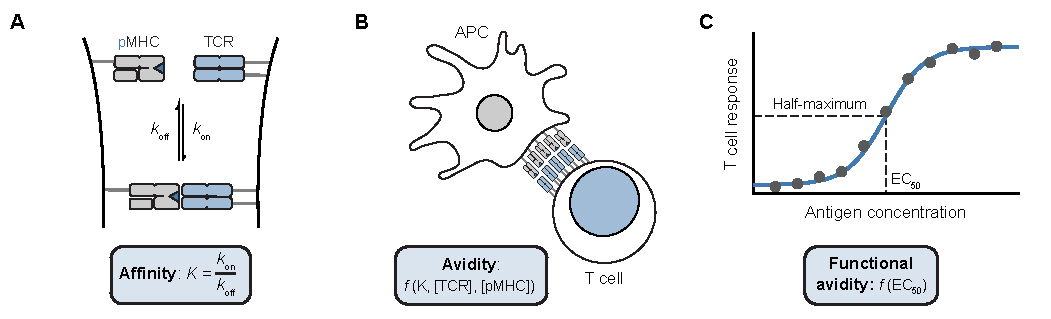
\includegraphics[width=\textwidth]{Figures/intro/fig6_affinityVsAvidity.pdf}
    \caption[Schematic depiction of TCR affinity, T cell avidity, and functional avidity]{%
    \textit{Schematic depiction of TCR affinity, T cell avidity, and functional avidity}. %
    %
    \secbfcolor{(A)}~TCR binding affinity for pMHC, denoted by $K$, is defined as the ratio between binding ($k_{\textup{on}}$) and unbinding ($k_{\textup{off}}$) rates. %
    %
    \secbfcolor{(B)}~T cell avidity is the cumulative binding strength that depends on the binding affinity of TCRs for pMHC, $K$, as well as on the surface densities of TCRs and pMHCs on the T cell and APC, respectively. %
    %
    \secbfcolor{(C)}~The functional avidity of the T cell is its measured sensitivity to pMHC, using readouts such as IFN-\textgamma{} production as a function of antigen concentration. It depends on the TCR:pMHC binding affinity, their respective surface densities, CD4/CD8 co-receptor expression, and other surface and intracellular signalling molecules that together modulate downstream T cell activation. Adapted from~\cite{this2021strength}.}
    \label{fig:intro_affinityVsAvidity}
\end{figure}

The fundamental interaction unit between a T cell and and an APC is the binding of one TCR to one pMHC; the  affinity of the TCR describes the strength of this unitary interaction. In a nutshell, the binding affinity represents the likelihood that a TCR ($T$) and pMHC ($P$) will remain in a bound state ($C$), and can be quantified via the equilibrium constant, $K$, of the following kinetic scheme (Fig.~\ref{fig:intro_affinityVsAvidity}A):
%
\begin{equation}
    \ch{$T + P$ <=>[$k\sb{\textup{on}}$][$k\sb{\textup{off}}$] $C$}.
\end{equation}
%
This equilibrium constant (also called the association constant) is a basic thermodynamic parameter, and is equal to the ratio between the binding and unbinding rates ($k_{\textup{on}}$ and $k_{\textup{off}}$, respectively), i.e., $K = \flatfrac{k_{\textup{on}}}{k_{\textup{off}}}$~\cite{stone2013role,margulies2001tcr}. The magnitudes of these kinetic parameters will be influenced by the TCR sequence, the MHC sequence, and the specific (self or foreign) peptide that is conjugated to the MHC~\cite{this2021strength}. Often, this quantity is given in terms of the dissociation constant, $K_D$~\cite{margulies2001tcr,martinez2015lower}, defined as the reciprocal of the association constant (i.e., $K_D = \flatfrac{1}{K}$).

It should be emphasized that, in reality, the binding affinity of a given TCR:pMHC pair depends on two independent parameters ($k_{\textup{on}}$ and $k_{\textup{off}}$) and each of these rates by themselves can have their own effect on TCR signalling. Indeed, Gálvez et al. showed, using a large collection of previously published T cell activation models based on the kinetic proofreading principle (see Section~\ref{sec:intro_overview_antigenDiscrimination}), that different values of $k_{\textup{on}}$ and $k_{\textup{off}}$ in almost all of these models can produce different outcomes, even if their ratio is fixed~\cite{galvez2019tcr}. It should therefore be borne in mind that, all else being equal, even two TCRs with the same measured affinity for a given pMHC may not necessarily lead to the same T cell response.

To obtain a direct measurement of TCR affinity and its associated kinetic parameters to a given pMHC, techniques such as isothermal titration calorimetry or surface plasmon resonance (SPR) have been used (reviewed in detail in~\cite{piepenbrink2009methods}). With SPR, different T cell clonotypes were found to have dissociation constants $K_D$ ranging from $\sim$0.1~\textmu{}M for high-affinity TCRs, up to the order of $100$~\textmu{}M for low-affinity TCRs~\cite{davis1998ligand,thomas2011human} (an appreciably large range spanning 4 orders of magnitude). These techniques have their share of disadvantages, however, with one being that they measure 3D binding affinities of free-floating, soluble TCRs when in fact TCR interaction with pMHC \textit{in vivo} is confined to 2D space across opposing T cell/APC membranes~\cite{martinez2015lower}. Alternative measures use techniques such as adhesion frequency and thermal fluctuation assays~\cite{huang2010kinetics} or single-molecule microscopy~\cite{huppa2010tcr} to determine binding affinities constrained to more realistic 2D environments; these 2D techniques indeed generate measurements with important differences when compared to their 3D counterparts~\cite{huang2010kinetics,huppa2010tcr,martinez2015lower}. A shortcoming associated with all of these techniques is that they cannot be used to measure affinity across all responding T cell clonotypes in a polyclonal response to a pathogen; rather, they are limited to measuring the affinity of one T cell clone or, at best, of T cell clonotypes with the same pMHC specificity.

%%%%%%%%%%%%%%%%%%%%%%%%%%%%%%%%%%%%%%%%%%%%%%%%%%%%
\subsection{T cell avidity -- a multi-dimensional gauge of pMHC reactivity}
\label{sec:intro_affinity_TcellAvidity}

While TCR affinity (and its corresponding kinetic parameters) certainly impact the strength of interaction between a T cell and an APC, scaling up from the molecular to the cellular level introduces additional layers of complexity. The propensity for T cells as a whole to bind an APC bearing cognate pMHC is termed its \textit{avidity}~\cite{this2021strength}. The magnitude of T cell avidity will depend on the binding affinity of one TCR:pMHC unit, together with the density of TCRs and pMHCs on the surfaces of the T cell and the APC, respectively (Fig.~\ref{fig:intro_affinityVsAvidity}B). Thus, a T cell with a fixed TCR surface density and a fixed binding affinity for a given pMHC may have different avidities for an APC depending on whether it expresses low, or high, levels of that cognate pMHC.

Staining of T cells using multi-valent, fluorescent pMHC compounds, or pMHC tetramers, is frequently used to quantify T cell avidity~\cite{christophersen2020peptide}. Given that the signal intensity will depend directly on the concentration of TCRs on the cell surface~\cite{christophersen2020peptide,wooldridge2009tricks}, pMHC tetramers only provide an indirect measure of its TCR affinity for the pMHC. Furthermore, tetramers have the misfortune of being less sensitive to T cells whose TCRs bind pMHC with low affinity, with one study showing that a large fraction of low-affinity responders are missed by tetramer staining altogether~\cite{andargachew2018cd4}. Furthermore, as with SPR or 2D affinity techniques, \textit{a priori} knowledge of T cell antigen specificity is needed to measure T cell avidity by tetramer staining, and use of tetramers to this effect may leave out important contributions from other T cells that recognize different pathogen-derived pMHC (known as different pMHC ``epitopes'').

The term T cell avidity is sometimes used interchangeably with \textit{functional avidity}~\cite{van2006t}, though these two quantities are not exactly the same. The functional avidity of a T cell will determine its overall antigen sensitivity by consolidating all factors involved in TCR signalling and T cell activation; in addition to binding affinity and receptor densities, functional avidity will also be affected by the co-receptors CD4 and CD8, co-stimulation, and the abundance and activity of downstream intracellular mediators that regulate positive or negative feedback mechanisms~\cite{this2021strength,james2022cd4,vigano2012functional,margulies2001tcr,slifka2001functional, viola1996t}. It is often measured \textit{in vitro} by assessing the production levels of effector cytokines such as IFN-\textgamma{}, T cell proliferation levels, or cytotoxic activity (i.e., the ability of CTLs to lyse target cells bearing cognate pMHC) as a function of antigen abundance or of target cell:CTL ratios~\cite{vigano2012functional} (Fig.~\ref{fig:intro_affinityVsAvidity}C). In all cases, the lower the antigen dose or the target cell:CTL ratio needed to illicit half the maximal response, the higher the relative functional avidity of that T cell. The term EC$_{50}$, borrowed from pharmacology nomenclature and used to discuss drug potency, is also sometimes used to describe this level associated with the response half-maximum~\cite{vigano2012functional}; the higher the EC$_{50}$, the lower the functional avidity of that T cell since more antigen is required to evoke a response.

Mathematical and computational population models of T cells, such as the one described in Section~\ref{sec:intro_overview_proliferation}, can incorporate functional avidity explicitly into their model equations. In Eq.~\eqref{eq:intro_deboer1995}, the parameter $K$ (not to be confused with the symbol for TCR affinity) was used to denote the functional avidity of the proliferating effector T cell population, with the quantity $\flatfrac{1}{K}$ representing the EC$_{50}$ (in the absence of clonal competition), i.e., the concentration of antigen inducing half-maximum proliferation. While T cell functional avidity is at best an approximation for the binding affinity of its TCR given the multi-factorial determinants of the former~\cite{margulies2001tcr}, these models may target such a parameter to specifically investigate the impact of TCR binding affinity on population dynamics if all other factors influencing functional avidity are assumed to be equal (or their differences negligible); this is the strategy we will employ in Chapter~\ref{sec:AvC}. In such cases, the term ``pMHC reactivity'' will be used to refer to changes in functional avidity as a direct result of differences in TCR:pMHC binding affinity.

%%%%%%%%%%%%%%%%%%%%%%%%%%%%%%%%%%%%%%%%%%%%%%%%%
\subsection{T cell reactivity to self- vs. foreign-pMHC}
\label{sec:intro_affinity_selfVsForeign}

Recall that the thymus trains and tolerizes T cells using a library of antigens derived from self. Thus, positive and negative selection in the thymus set the lower and upper bounds, respectively, of how reactive T cells may be at least in the context of \textit{self}-pMHC. It was shown that the strength of TCR interaction with self-pMHC correlates with expression levels of CD5 on both CD4\pos{}~\cite{azzam1998cd5,mandl2013t} and CD8\pos{}~\cite{fulton2015tcr} T cells. CD5 is a surface molecule on T cells that serves as a negative regulator of TCR signalling~\cite{tarakhovsky1995role,hawiger2004immunological}; interestingly, it was shown that na\"{i}ve CD4\pos{} T cells with higher levels of CD5 expression (i.e., CD5\supr{hi} CD4\pos{} T cells), thus having higher reactivity to self-pMHC, also bind \textit{foreign}-pMHC more strongly than their CD5\supr{lo} counterparts, on average~\cite{mandl2013t,rogers2021pre}. It can be noted that CD8\pos{} T cells, on the other hand, possess narrower distributions of CD5 expression levels~\cite{azzam1998cd5,mandl2013t} that do not correlate with foreign-pMHC binding strength~\cite{fulton2015tcr} as seen in CD4\pos{} T cells. However, there is evidence to suggest that a relationship does indeed also exist between self- and foreign-pMHC binding strengths in CD8\pos{} T cells; for example, in one study, it was shown that when mutations were introduced in a TCR that increased its binding affinity for cognate pMHC, its affinity for self-pMHC also increased~\cite{holler2003tcrs}.

Ultimately, the ability for a TCR to bind pMHC will rely both on its binding strength to the (self- or foreign-) peptide, but also to the MHC molecule itself. To study the relationship between foreign-pMHC recognition and self-pMHC affinity in T cells undergoing positive and negative selection in the thymus, theoretical ``digit-string'' models have been developed that represent the TCRs and the pMHC as strings of random numbers~\cite{detours1999explaining,detours2000paradox,chao2005effects}. In these models, the binding contributions from the peptide itself and from the MHC molecule to the TCR were assumed to be distinct and independent from each other (Fig.~\ref{fig:intro_digitString}). The binding affinity is then taken as being proportional to the degree of overlap between these two strings, with positive and negative selection setting the lower and upper bounds, respectively, of the self-pMHC binding affinities of the TCR repertoire. Using one such model, Chao et al. showed that, in some cases, there can indeed be a relationship between self- and foreign-pMHC affinities. In fact, they argued that such TCRs would require lower binding contribution from the MHC to survive selection, and that they are thus more specific (i.e., less cross-reactive) than TCRs where the MHC contributes predominantly to TCR binding~\cite{chao2005effects}.
%
\begin{figure}
    \centering
    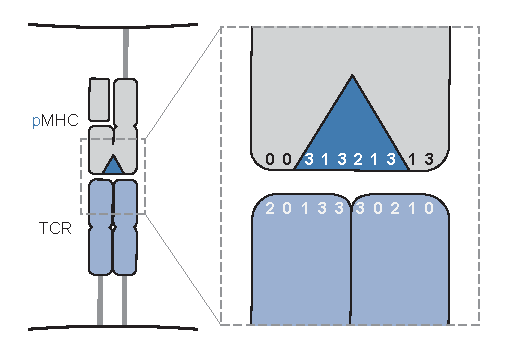
\includegraphics[width=0.48\textwidth]{Figures/intro/fig7_digitString.pdf}
    \caption[Digit-string representation of TCR:pMHC binding affinity]{%
    \textit{Digit-string representation of TCR:pMHC binding affinity}. %
    %
    The binding domains of the TCR, the peptide, and the MHC are modelled as a string of random numbers between 0 and 127 (only 0 to 3 shown here), with the affinity being proportional to the similarity between the TCR string and the compound peptide-MHC string. Adapted from~\cite{chao2005effects}.}
    \label{fig:intro_digitString}
\end{figure}

%%%%%%%%%%%%%%%%%%%%%%%%%%%%%%%%%%%%%%%%%%%%%%%%%
\subsection{Low-avidity T cells -- unsung heroes?}
\label{sec:intro_affinity_highVsLowAffinity}

Given their greater sensitivity to pMHC by definition, it is perhaps unsurprising that many groups have reported that T cells with higher foreign-pMHC reactivity predominantly respond to infection~\cite{busch1999t,king2012t,rosenthal2012low,mandl2013t,straub2023recruitment}. Indeed, in multi-clonal T cell population models where the probability of proliferation is higher for higher-avidity T cells, these cells outnumber their lower-avidity counterparts upon antigen-driven clonal expansion~\cite{de1994t,de1995towards,chao2004stochastic,chao2004modelling}. However, T cells that possess lower-affinity TCRs are known to also contribute to anti-microbial responses~\cite{martinez2015lower,martinez2016low,kolawole2020relationship}. Additionally, since autoreactive low-avidity T cells specific for self-pMHC predominantly escape negative selection and can cause autoimmunity as discussed in Section~\ref{sec:intro_autoimmunity_whyCentralAndPeripheral}, it follows that these T cells indeed possess the effector potential necessary to carry out immune responses~\cite{kolawole2020relationship}. Furthermore, emerging evidence suggests that, in both CD4\pos{} and CD8\pos{} T cells, those with lower-affinity TCRs may predominate in the case of chronic infection where the pathogen persists for extended periods of time within the host~\cite{gallegos2016control,tsitsiklis2020unusual,schober2020reverse}. However, given the difficulty in detecting these T cells (let alone assessing their function) within a polyclonal population using conventional experimental techniques, computational modelling can be a useful tool to investigate their contribution in controlling pathogen replication (Chapter~\ref{sec:AvC}). 

%%%%%%%%%%%%%%%%%%%%%%%%%%%%%%%%%%%%%%%%%%%%%%%%%
\subsection{Summary and highlights}
The peripheral pool of pathogen-specific T cells is composed of a TCR repertoire that may bind pathogen-derived pMHC across a wide range of affinities, with both low- and high-affinity T cells contributing to the response. However, to date there does not exist any perfect experimental technique that can simultaneously and comprehensively measure the affinity of all pathogen-specific TCR clonotypes across this large continuum. Specifically, T cells with low foreign-pMHC binding strength are often overlooked or go undetected, yet they may be important contributors to the anti-pathogen immune response. In Chapter~\ref{sec:AvC}, we used modelling to complement experimental techniques, with the goal of investigating the function of these T cells with lower pMHC binding strengths and how infection duration (i.e., chronic vs. rapidly cleared ``acute'' infections) might play a role.

%%%%%%%%%%%%%%%%%%%%%%%%%%%%%%%%%%%%%%%%%%%%%%%%%
%%%%%%%%%%%%%%%%%%%%%%%%%%%%%%%%%%%%%%%%%%%%%%%%%
\section{T cell escape}
\label{sec:intro_immuneEscape}

Over the course of an infection, what T cells will ``see'' is often not static. In fact, many pathogens have independently and remarkably evolved mechanisms to acclimate to their environment within the host and avoid detection by T cells in a process known as ``immune evasion''  or ``escape''. Pathogens do this in large part by manipulating the ability of TCRs to bind to their respective pathogen-derived pMHCs, thereby ``blinding'' T cells, in a sense, to their presence and preventing them from carrying out their anti-microbial responses. Thus, a tug-of-war exists between T cells and pathogens as the latter attempt to adapt to selective pressure exerted by the former. Notably, there are a large number of different strategies that pathogens may employ to evade detection or clearance by pathogen-specific T cell populations, and these will vary depending on the type of pathogen in question. While there is an entire branch within the field of microbiology dedicated to understanding the inner workings of these mechanisms, for the purposes of this thesis, I will provide only a broad overview of such strategies. 

%%%%%%%%%%%%%%%%%%%%%%%%%%%%%%%%%%%%%%%%%%%%%%%%%
\subsection{Mechanisms of T cell escape}
\label{sec:intro_immuneEscape_mechanisms}

The first common mechanism of immune escape worth discussing is the concept of ``dormancy'' or ``quiescence'', whereby bacterial pathogens such as \textit{Mycobacterium tuberculosis}, as well as some fungal pathogens, can enter states of non-reproduction and non-infectivity in order to ``hide'' from the host~\cite{rittershaus2013normalcy,shepherd2020t,brunet2018reactivation}. Though the underlying microbiological pathways are distinct, viruses can behave in a similar manner in a process known as viral ``latency'', where the viral genome resides within the host cell but suspends the production of new viral particles; this latent virus remains replication-competent in spite of its apparent dormancy, allowing it to become re-activated after potentially long times (even years)~\cite{speck2010viral,eshleman2011varicella,delannoy2019cat,zangger2022t}. In fact, the ability of human immunodeficiency virus (HIV) to be so elusive to anti-retroviral treatments is in no small part due to the presence of its latent reservoir of infected cells~\cite{chun1999latent,delannoy2019cat}. The dynamics of HIV infection have been modelled extensively (reviewed in~\cite{perelson2002modelling,rong2009modeling,hill2018mathematical}), and inclusion of these latent reservoirs in such models indeed demonstrated decreased likelihood for the potential of anti-retroviral therapies to achieve viral eradication in infected individuals.

Another mechanism adopted by a range of viral and intracellular bacterial pathogens to avoid detection by T cells is the induction of MHC class I (MHCI) downregulation~\cite{hewitt2003mhc,shepherd2020t,delannoy2019cat,antoniou2008pathogen}. Again, the molecular mechanisms employed to this effect are complex and heterogeneous (reviewed in~\cite{antoniou2008pathogen}), but generally speaking, they all serve to reduce recognition by CD8\pos{} T cells since these require interaction with pathogen-derived pMHC expression via their TCR to clear infected cells. \textit{Plasmodium} protozoa, the parasites responsible for malaria, also induce MHCI downregulation within infected Kupffer cells in the liver during the sporozoite stage of their life cycle~\cite{steers2005immune,gomes2016immune}. Additionally, these parasites have the advantage that, during their later merozoite stage, they infect anucleate red blood cells (RBCs) that do not express any MHC at their cell surface, thus impairing the ability of CD8\pos{} T cells to find and kill infected cells~\cite{gomes2016immune}. Furthermore, pathogens may take advantage of peripheral tolerance mechanisms whose aim is to suppress T cell responses~\cite{garib2015t} (see Section~\ref{sec:intro_autoimmunity_peripheralTolerance}). For example, they may alter APC function to induce the differentiation of pathogen-specific conventional T cells into immunosuppressive regulatory T cells such as Tr1 cells~\cite{belkaid2007regulatory,belkaid2009regulatory,garib2015t,boer2015regulatory}. In a similar vein, chronic stimulation of pathogen specific CD4\pos{} and CD8\pos{} T cells can drive functional exhaustion in these T cells. This exhausted phenotype is characterized by the loss of the ability of these T cells to carry out their anti-microbial functions, such as production and release of their signature pro-inflammatory cytokines or cytotoxic responses~\cite{zajac1998viral,wherry2011t,shepherd2020t}.

One T cell evasion strategy of particular relevance for this thesis is the concept of ``antigenic variation''. Briefly, antigenic variation entails genetic or epigenetic modifications that effectively alter what will be presented to T cells in the context of pMHC~\cite{deitsch2009common}. The former might involve mutations or recombination in the pathogen genome, while the latter refers instead to changes in their gene expression patterns. More complex microorganisms, such as bacteria, fungi, and protozoa, have evolved fairly intricate mechanisms of antigenic variation, including phase variation (switching individual genes between ``on'' and ``off' 'states) and mutually exclusive expression (alternating which genes from a large multi-copy gene family is actively transcribed), among others~\cite{van2004phase,deitsch2009common,florini2022shared}. Viruses, being much simpler microorganisms\footnote{Viruses are technically not microorganisms since they are not self-sustaining and not officially considered ``living'', though there is some debate around this~\cite{brown2016viruses}.} with much smaller (DNA or RNA) genomes that completely rely on the cellular machinery of the host cells they infect to sustain themselves and to reproduce, employ a different strategy. In fact, viruses (in particular RNA viruses such as HIV, but also DNA viruses to a lesser extent) have very high mutation rates originating in large part (though not exclusively) from genome replication errors~\cite{sanjuan2016mechanisms}. While most of these mutations are deleterious or even lethal for the virus~\cite{domingo2009fitness,wylie2011biophysical}, some might provide an adaptive advantage with one possible benefit being mutations in pMHC epitope regions of the viral genome, and thus T cell escape (Fig.~\ref{fig:intro_antigenicVariation}).

\begin{figure}
    \centering
    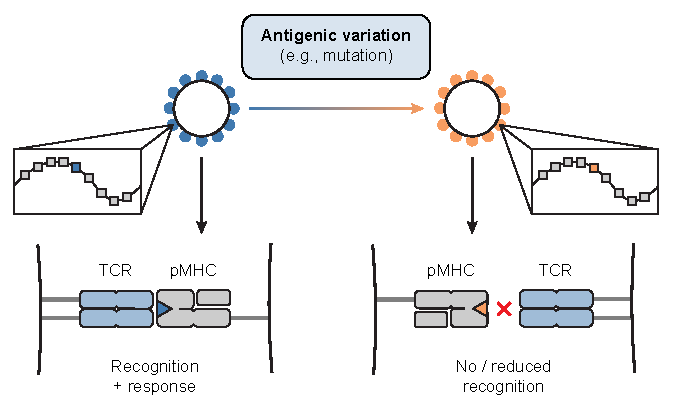
\includegraphics[width=0.64\textwidth]{Figures/intro/fig8_antigenicVariation.pdf}
    \caption[Antigenic variation as a mechanism of T cell escape]{\textit{Antigenic variation as a mechanism of T cell escape}. %
    %
    Some pathogens can undergo modifications (e.g., mutations as is typically the case for viruses, shown here) that alter what T cells will see via their TCR. Schematic insets depict a single amino acid substitution in the peptide sequence that becomes conjugated to the MHC molecule, thus altering the pMHC epitope. Antigenic variation can lead to an impaired capacity of the TCR to bind the altered pMHC, thus reducing or eliminating the ability of those T cells to respond to (and clear) the pathogen.}
    \label{fig:intro_antigenicVariation}
\end{figure}

\subsection{Within-host pathogen evolution -- lessons from RNA viruses}

RNA viruses that produce chronic infections within their host, such as HIV and hepatitis C virus (HCV), possess a remarkable capacity to evolve escape mutations in pMHC epitope regions of their genome, thus evading the anti-viral T cell response~\cite{weiner1995persistent,borrow1997antiviral}. This follows from the fact that, relative to all other microorganisms, RNA viruses have the highest replication error rate per nucleotide within their genome~\cite{peck2018complexities,sanjuan2016mechanisms}. Given the high propensity for these viruses to mutate with every replication cycle, together with short generation times and massive amounts of new virions being formed daily within an infected host (e.g., at least 10 billion per day in HIV as estimated from mathematical population models~\cite{perelson1996hiv,perelson2002modelling}), a viral population in biological systems is almost always comprised of a large collection of unique genomes; thus, the term ``quasispecies'' is used to describe such populations~\cite{andino2015viral,domingo2019viral,lauring2020within}.

\begin{figure}
    \centering
    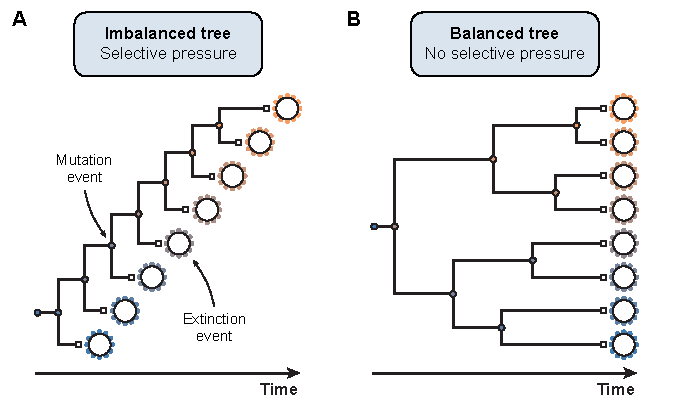
\includegraphics[width=0.64\textwidth]{Figures/intro/fig9_phylodynamics.pdf}
    \caption[Idealized representation of within-host phylodynamic tree topologies]{%
    \textit{Idealized representation of within-host phylodynamic tree topologies}. %
    %
    \secbfcolor{(A)}~Imbalanced (or ladder-like) tree architecture representing pathogen evolution under strong selective pressure. %
    %
    \secbfcolor{(B)}~Balanced (or star-like) tree architecture occurring in the absence of selective pressure on pathogen evolution. Adapted from~\cite{volz2013viral}.}
    \label{fig:intro_phylodynamics}
\end{figure}

Assessing the composition of viral quasispecies, and how they evolve over the course of an infection within a host, can be done using a combination of sequencing approaches and phylogenetic analyses~\cite{volz2013viral,lauring2020within}. ``Phylodynamic'' trees are often used to study the intersection between immunological and epidemiological processes that shape pathogen evolution within hosts (our interest for the purposes of this thesis) and also at the between-host/population scales~\cite{grenfell2004unifying,bons2018virus}; the latter will be revisited in Chapter~\ref{sec:conclusion} when discussing extensions and possible implications of our within-host studies. One example of the use of phylodynamic trees is that they can inform the evolutionary pressures present on the replicating pathogen, where imbalanced or ``ladder-like'' tree topologies reveal strong selection pressures influencing viral adaptation as compared to balanced trees (Fig~\ref{fig:intro_phylodynamics})~\cite{grenfell2004unifying,volz2013viral}. At the within-host level, these imbalanced trees have indeed revealed strong selection pressures shaping HIV and HCV evolution~\cite{grenfell2004unifying,raghwani2019high,lemey2006hiv}.

Influenza A virus (IAV) is another RNA virus with fairly high mutation rates~\cite{sanjuan2010viral}. While \textit{de novo} mutations do arise in infected hosts, when compared to HIV or HCV, IAV within-host evolution is limited by the fact that these viruses are usually cleared by the immune system within 5-7 days post-infection (as estimated from mathematical modelling of viral load kinetic data)~\cite{xue2018within,baccam2006kinetics}. However, in immunocompromised individuals where the infection may last much longer (weeks or months), extensive evolution and antigenic variation has been measured by longitudinal viral sampling of these hosts~\cite{rocha1991antigenic,mcminn1999antigenic,xue2017parallel}. Given the consequences that viral evolution within infected hosts may have on the epidemiology and spread of infectious diseases, studying how T cell-mediated immunity can shape this evolutionary process remains of utmost importance.

%%%%%%%%%%%%%%%%%%%%%%%%%%%%%%%%%%%%%%%%%%%%%%%%%
\subsection{Pathogen-immune co-evolution -- the role of T cell selective pressure}
\label{sec:intro_immuneEscape_RNAviruses}

As T cells play a fundamental role in orchestrating anti-microbial responses, it follows that they act as a major driver of within-host pathogen evolution by exerting strong selection pressures and shaping fitness landscapes that the pathogen must exploit in order to persist. While longitudinal viral sequencing studies can provide valuable information into how these pathogens are evolving over time within their host, simultaneously assessing the complimentary and dynamic role that T cells play in driving these changes using experimental techniques is challenging. Modelling efforts are thus needed to gain insight into how T cells and pathogens interact with one-another to generate outcomes observed from monitoring viral sequences. In 2004, Grenfell et al. described a simple conceptual model of how the balance between pathogen control and immune selection pressure may ultimately shape within-host pathogen evolution and the ensuing phylodynamic patterns observed for different viruses~\cite{grenfell2004unifying}. In their model, the number of advantageous mutations (and thus the propensity for the virus to adapt) results from a necessary combination of sufficient viral abundance and immune pressure favouring these mutations (Fig.~\ref{fig:intro_abundanceVsPressure}). This model formalism predicted a ``sweet spot'' where the product of these two quantities results in maximal potential for the virus to adapt under selection pressures exerted by the immune system.

\begin{figure}
    \centering
    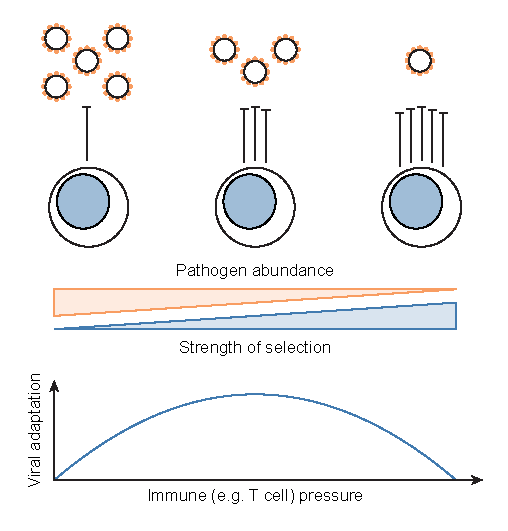
\includegraphics[width=0.48\textwidth]{Figures/intro/fig10_abundanceVsPressure.pdf}
    \caption[Conceptual model of viral adaptation as a function of immune pressure]{%
    \textit{Conceptual model of viral adaptation as a function of immune pressure}. %
    %
    Higher levels of immune-mediated control on viral replication decrease the abundance of the pathogen, but increase the strength of selection favouring viral evolution/adaptation to the host environment. The propensity for the virus to adapt is taken as a product of these two factors and peaks at intermediate immune pressures. Adapted from~\cite{grenfell2004unifying}.}
    \label{fig:intro_abundanceVsPressure}
\end{figure}

To study how HIV-T cell co-evolution and the production of new antigenic variants of the former leads to the eventual failure of T cells to control HIV replication and subsequently to the development of acquired immunodeficiency syndrome (AIDS), Nowak et al. developed a mathematical population model where unique variants of HIV, and their associated T cell responses, were explicitly distinguished from each other~\cite{nowak1991antigenic}. In their model, the probability that a new antigenic variant arises was taken to be proportional to HIV viral loads, which were negatively modulated by the responding T cell population. Based on their model formalism, they found that once the number of HIV variants exceeds a critical threshold, T cells specific for these antigens become overwhelmed and are no longer able to keep viral loads in check, leading to the onset of AIDS. In another model of HIV evolution and CTL escape, van Deutekom et al. showed that slow accumulation of escape mutations during the clinical latency phase of HIV infection leads to an eventual rise in the rate of escape at late stages of infection, which in turn drives higher viral loads and further amplifies the emergence of new mutants in a positive feedback loop until complete T cell escape is achieved~\cite{van2013rate}. While these models have certainly generated informative and useful insights, there is still a need to study more specific aspects of the the T cell response and how these in turn can modulate the ability of a pathogen to evolve within the host.

\subsection{Summary and highlights}

While T cells are indispensable for choreographing immune responses to pathogens, their anti-microbial functions exert a selective pressure that many pathogens have evolved to exploit, resulting in T cell escape and impaired control of pathogen replication. The potential consequences of this constant tug-of-war are all-too-familiar to us, having just lived through a pandemic where viral adaptation evidently led to the emergence of many pathogen variants that evaded pre-existing immunity and greatly complicated efforts to contain their spread. Thus, there is an imperative need for us to better understand how specific aspects of the T cell response can modulate the rates of immune escape. In Chapter~\ref{sec:VE}, we will study how TCR repertoire diversity might affect this balance between pathogen control and adaptation, by asking whether less diverse TCR repertoires might exacerbate the capacity of these pathogens mutating within their hosts to generate variants that escape T cell recognition.